%!TEX root = ../report.tex

% 
% Related work
% 

\section{Related Work}
\label{sec:related_work}

After that we give an overview of the related work that has been carried out on procedural generation of large amounts of geometry.

Since the target audience of this work are architects and designers, most of the work that we present have the same target.

\subsection{Procedural Modeling Tools} % (fold)

The following two sections are presented tools that use different techniques of procedural generation applied to the modeling of urban environments.

%!TEX root = ../../report.tex

\subsection{CityEngine \cite{Parish2001} \cite{Muller2006}}
\label{sub:cityengine}

CityEngine is a three-dimensional (3D) modeling software developed by Procedural Inc. (now part of the Esri R\&D Center). Specialized in the generation of 3D urban environments. With the procedural modeling approach, CityEngine enables the efficient creation of detailed and large-scale 3D city models with a lot of control from the user. This system applies the concept of Immediate Feedback by allowing the user to immediately see the results of each change. This is implemented through a set of sliders that are assigned to various indicators in the model that can be as high level as the \emph{size of the city} or as specific as the width of the windows or the number of floors in a building.

The following sections explain how CityEngine faces each of the steps in the generation of a city, such as road network generation or building modeling.

\begin{figure}[htbp]
  \centering
  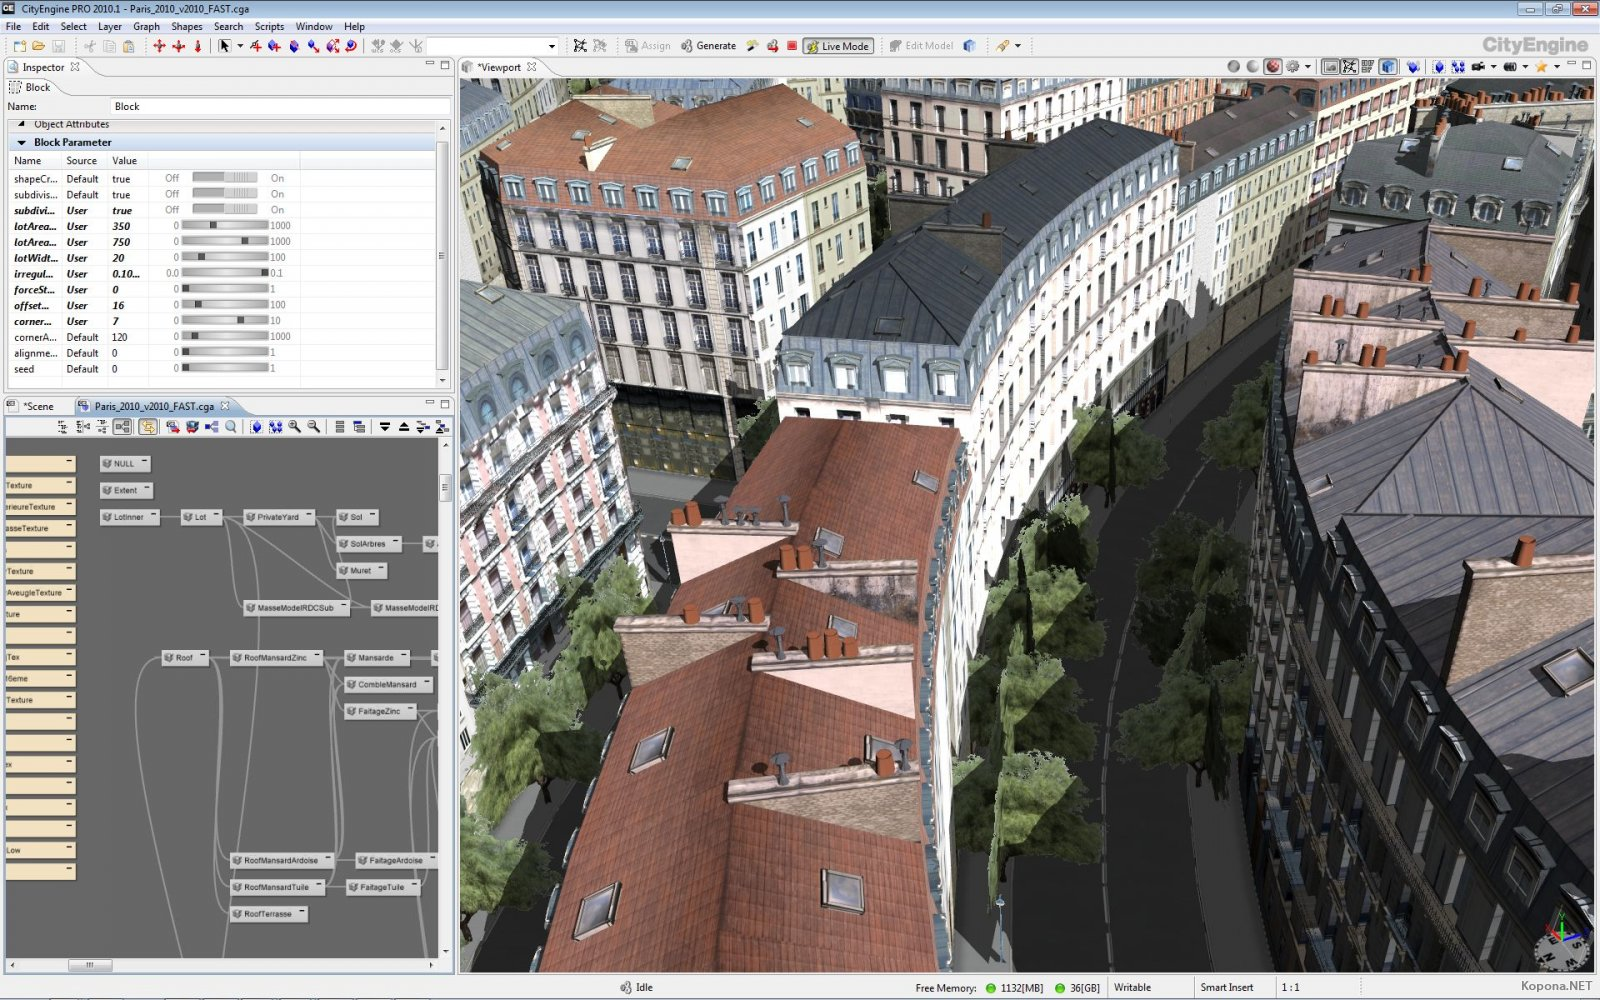
\includegraphics[width=\textwidth]{img/Procedural-Modeling-of-Cities/interface.jpg}
  \caption{City Engine Interface}
  \label{fig:CEinterface}
\end{figure}

\subsubsection{RoadNetwork} % (fold)
\label{ssub:roadnetwork1}


The first part to procedurally generate a city is to create a road network to become a backbone of the city and provide an overall structure. For that, CityEngine receives as input maps such as land-water boundaries and population
density. From that input a network of highways is created to connect the areas off high density population, and small roads connect to the highways.
This growth process continues until the average area of each lot is the desired one. The system have a default value, but it can be set by the user to a different one.

To implement this growth process, it uses an L-System (Section~\ref{ssub:l_systems}) that computes the road network.


\begin{figure}[htbp]
  \centering
  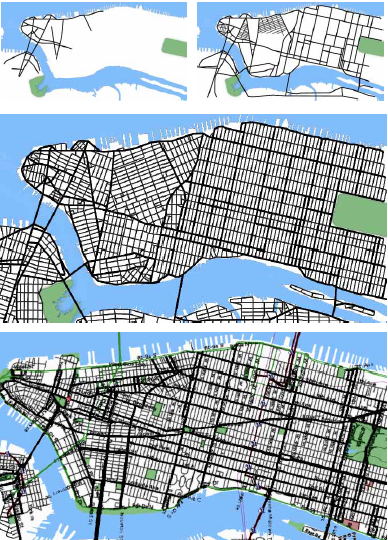
\includegraphics[width=0.5\textwidth]{img/Procedural-Modeling-of-Cities/Capturar.png}
  \caption{Road Map growth}
  \label{fig:city}
\end{figure}

The Figure~\ref{fig:city} shows the evolution of this process in a map of Manhattan. The first two pictures on the top shows the process in different phases during the process, the picture in the middle is the result of the process and the bottom line is the real map of Manhattan for comparison.

% subsubsection roadnetwork (end)Road Network

\subsubsection{Buildings} % (fold)
\label{ssub:buildings1}

To implement the generation of buildings, CGA was created, which is a shape grammar(Section~\ref{ssub:shape_grammars}) that was introduced in \cite{Parish2001}. It is defined as ``a novel shape grammar for the procedural modelling of CG architecture, produces building shells with high visual quality and geometric detail." To do so, this grammar uses a group of well defined production rules.

This tool allows the user to model buildings with an high control and in different ways. It can be done by text, writing production rules from a shape grammar or with a visual language similar Grasshopper 3D, that is nice for simple models but it is hard to work with more complex models, for instance, Figure~\ref{fig:CEinterface} shows a set of rules (bottom left), that is relatively small but is already difficult to follow the connections between rules.

\paragraph{Mass Modeling} % (fold)
\label{par:mass_modeling}
To model a building the first step is to create a mass model of the entire building by assembling basic shapes. With scaling, translation rotation and split applied to basic shapes namely I, L, H, U and T as shown in the Figure~\ref{fig:basic_shapes}.

\begin{figure}[htbp]
  \centering
  
\includegraphics[width=0.95\textwidth]{img/Procedural-Modeling-of-Cities/MassModeling2.png}
  \caption{Basic shapes}
  \label{fig:basic_shapes}
\end{figure}

% paragraph mass_modeling (end)

The next step is to add the roof, from a set of basic roof shapes or general L-Systems.

After that, with the application of the grammar rules in the created mass, it is possible to create complexity to the level that is desired, being able to produce highly complex buildings like the one in Figure~\ref{fig:CEnewbuilding}.


\begin{figure}[htbp]
  \centering
  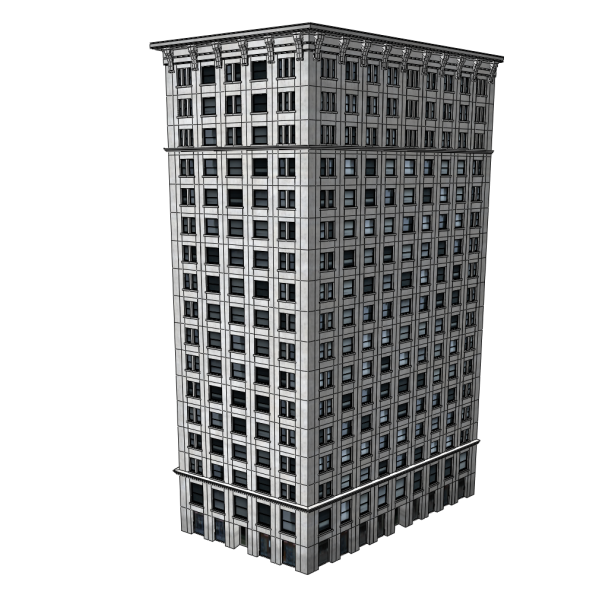
\includegraphics[width=0.8\textwidth]{img/Procedural-Modeling-of-Cities/building2.png}
  \caption{Complex building modeled with CGA}
  \label{fig:CEnewbuilding}
\end{figure}

% subsubsection buildings (end)

\subsubsection{Cities} % (fold)
\label{ssub:Cities1}

The result can be a city like Figure~\ref{fig:bigCity}, with approximately 26000 buildings.

\begin{figure}[htbp]
  \centering
  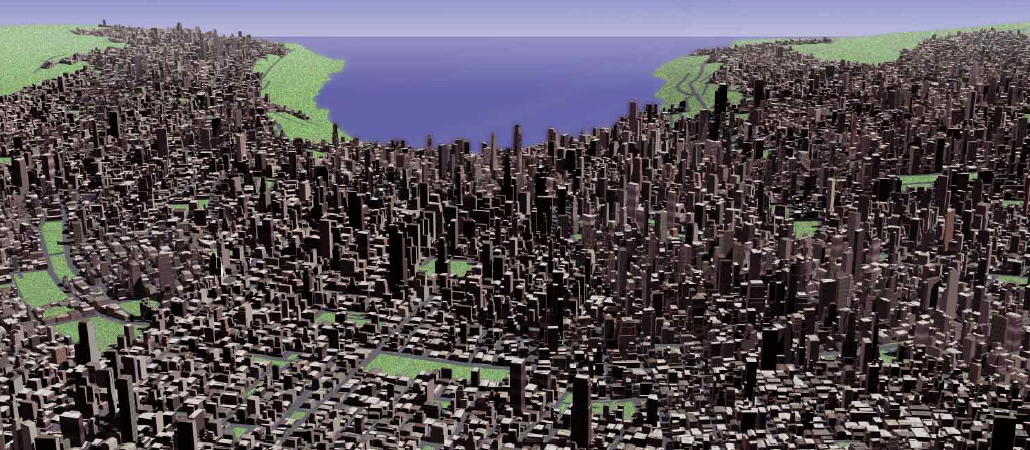
\includegraphics[width=0.95\textwidth]{img/Procedural-Modeling-of-Cities/City.png}
  \caption{City with approximately 26000 buildings.}
  \label{fig:bigCity}
\end{figure}

City Engine outputs can be imported by Maya\footnote{\url{http://www.autodesk.com/products/maya/overview}}, to achieve better results. Like the Figure~\ref{fig:cityMaya}, that represents a ‘virtual’ Manhattan.

\begin{figure}[htbp]
  \centering
  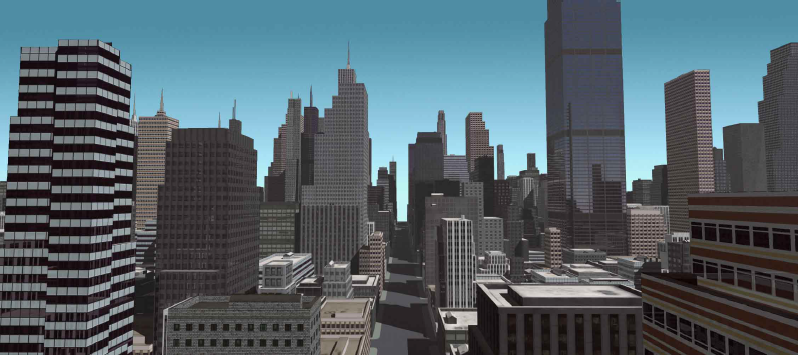
\includegraphics[width=0.95\textwidth]{img/Procedural-Modeling-of-Cities/City_Maya.png}
  \caption{City rendered with Maya.}
  \label{fig:cityMaya}
\end{figure}

% subsubsection subsubsection_name (end)

%!TEX root = ../../report.tex

\subsection{Undiscovered City} % (fold)
\label{sub:undiscovered_city}

In \cite{Greuter2003} Stefan Greuter et al. presented a system that generates in real-time pseudo infinite virtual cities which can be interactively explored from a first person perspective. In their approach ``all geometrical components of the city are generated as they are encountered by the user." As shown in the Figure~\ref{fig:viewingRange} only the part of city that is inside the viewing range is generate. This method allows the visualization of massive amounts of geometry, buildings in this case, by generating in real time only the geometry that on sight, and since this subset is usually much smaller than all the geometry this results in huge benefits in performance.

\begin{figure}[htbp]
	\centering
	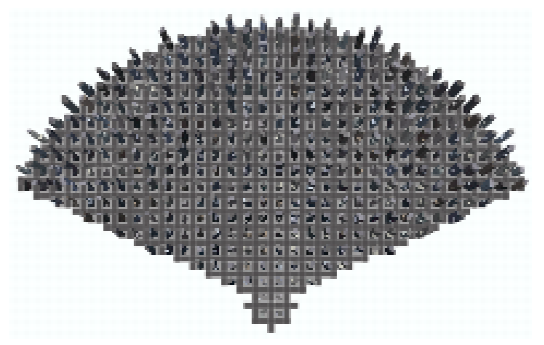
\includegraphics[width=0.85\textwidth]{img/Real-Time-procedural-generation/viewing-range.png}
	\caption{Viewing Range}
	\label{fig:viewingRange}
\end{figure}

\subsubsection{Road Network} % (fold)
\label{ssub:road_network}

The system uses a 2D grid that divide the terrain into square cells. The cells represent proxies for the content that will be procedurally generated. Before the content of each cell is generated, the potential visibility of it is tested, and after that, only the visible cells are filled with content.

Then the roads are created in a uniform grid pattern. This grid does not feel very natural, and in the continuation of the work, this system evolved into a more realistic one with the join of some of the grids to create a less uniform distribution of the buildings.

% subsubsection road_network (end)

\subsubsection{Buildings} % (fold)
\label{ssub:buildings}


To compute the form and appearance of each building, it is used a ``single 32 bit pseudo random number generator seed. The random sequence determines building properties such as width, height and number of floors."
Similar sequences of number result in similar buildings. To avoid that, it is used a a hash function to convert each cell position into a seed.

To generate a building the first is to generate a floor plan. To do so, it is randomly selected and merged a set of regular polygons and rectangles, then this is extruded. This is an iterative process, that creates sections from the top to the bottom, by adding more shapes to the the initial shape and extruding as shown in the Figure~\ref{fig:UC_buildings}. Starting from the left, first there is a simple polygon, that is merged with a rectangle and after extrusion, forms the first block that will be the top of the building. After that, another extrusion is made to generate the next block followed by the merge of a rectangle to the floor shape and the generation of a new block and so on.

\begin{figure}[htbp]
	\centering
	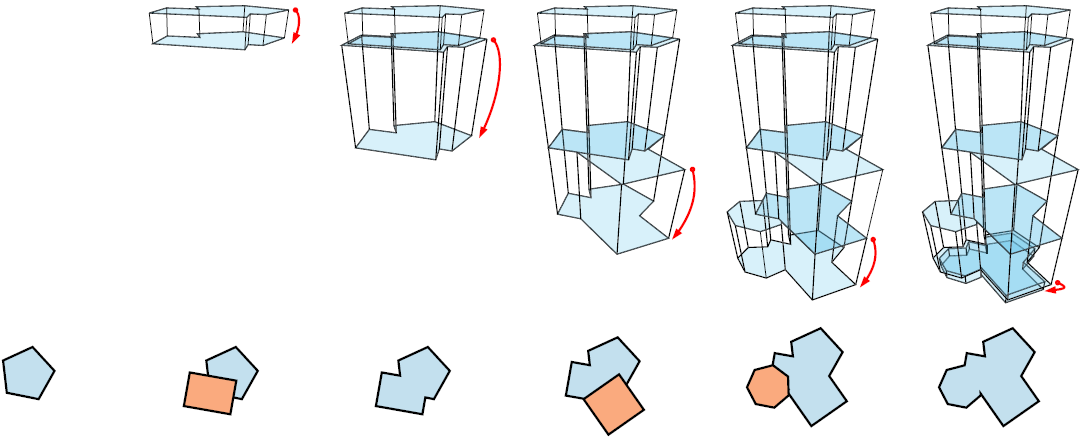
\includegraphics[width=0.85\textwidth]{img/Real-Time-procedural-generation/Building-Generation.png}
	\caption{buildings}
	\label{fig:UC_buildings}
\end{figure}

With the application of this method very complex architectural forms can be generated, depending only on which forms are selected and the order that is used to merge them.

% subsubsection buildings (end)

% subsection undiscovered_city (end)



\subsection{Conclusion} % (fold)
\label{sub:conclusion}

The presented procedural modeling techniques are important for the procedural generation of geometry, such as Fractals (Section~\ref{ssub:fractals}), and Noise (Section~\ref{ssub:noise}), and will be supported and may even applied during the development of this work. Additionally, techniques related to visualization, such as level of detail (Section~\ref{ssub:level_of_detail}), was presented and will be explored to help improve performance.

The systems presented (Section~\ref{sub:cityengine},Section~\ref{sub:undiscovered_city}) show ways to generate and visualize large volumes of geometry, in this cases applied to urban models. While CityEngine \cite{Parish2001} aims to allow the users to create large and realistic urban models, where they give, in the limit, total control to the users. Undiscovered City\cite{Greuter2003} is much more a visualization tool, it generates the model automatically for the user to explore.

From these works there are some ideas to explore. The idea of immediate feedback that is implemented in CityEngine, with sliders, is a good input to our work. This helps the unexperienced users to easily see the how their code impact the results. Also the commands they have on the grammar could be an helpful inspiration for the design of our API.

From the Undiscovered City system, since they also have massive amount of geometry, how they tackle this problem is very important source of inspiration as well.

% subsection graphic_tools (end)

% subsection conclusion (end)

